\PassOptionsToPackage{utf8}{inputenc}
\documentclass{bioinfo}
\copyrightyear{2015} \pubyear{2015}

\access{Advance Access Publication Date: Day Month Year}
\appnotes{Manuscript Category}



%%% PACKAGES

\usepackage{xr}
\externaldocument{RNARedPrint-Bioinfo2018}


\usepackage{booktabs} % for much better looking tables
\usepackage{array} % for better arrays (eg matrices) in maths
% \usepackage{paralist} % very flexible & customisable lists (eg. enumerate/itemize, etc.)
%   \let\itemize\compactitem
%   \let\enditemize\endcompactitem
%   \let\enumerate\compactenum
%   \let\endenumerate\endcompactenum
%   \let\description\compactdesc
%   \let\enddescription\endcompactdesc
%   \pltopsep=1pt
%   \plitemsep=1pt
%   \plparsep=1pt  
\usepackage{hyperref} 
\usepackage{xspace} 
%\usepackage{geometry} 
\usepackage{amsmath,amssymb} 
\usepackage{bm}
\usepackage{verbatim}
\usepackage{longtable}
\usepackage[vlined]{algorithm2e}

\usepackage{xifthen}
\usepackage{stmaryrd}

\usepackage{xcolor}


\hypersetup{
    bookmarks=false,         % show bookmarks bar?
    unicode=false,          % non-Latin characters in Acrobat’s bookmarks
    pdftoolbar=true,        % show Acrobat’s toolbar?
    pdfmenubar=true,        % show Acrobat’s menu?
    pdffitwindow=true,     % window fit to page when opened
    pdfstartview={FitH},    % fits the width of the page to the window
    colorlinks=true,       % false: boxed links; true: colored links
    linkcolor=red!70!black,          % color of internal links (change box color with linkbordercolor)
    citecolor=blue!50!black,        % color of links to bibliography
    filecolor=magenta,      % color of file links
    urlcolor=green!50!black           % color of external links
}


%%%%%%%%%%%%%%%%%%%%%%%%%%%%%%%%%%%%%%%%
%% Rolf's includegraphicstop
\makeatletter
\newsavebox{\@alignepsbox}
\newlength{\@aligneps}
\newcommand{\includegraphicstop}[2][]{%
\sbox{\@alignepsbox}{\includegraphics[#1]{#2}}%
\setlength{\@aligneps}{-\ht\@alignepsbox}%
\addtolength{\@aligneps}{2ex}%
\raisebox{\@aligneps}{\usebox{\@alignepsbox}}}
\makeatother


%\makeatletter
%\let\oldlt\longtable
%\let\endoldlt\endlongtable
%\def\longtable{\@ifnextchar[\longtable@i \longtable@ii}
%\def\longtable@i[#1]{\begin{figure}[t]
%\onecolumn
%\begin{minipage}{0.5\textwidth}
%\oldlt[#1]
%}
%\def\longtable@ii{\begin{figure}[t]
%\onecolumn
%\begin{minipage}{0.5\textwidth}
%\oldlt
%}
%\def\endlongtable{\endoldlt
%\end{minipage}
%\twocolumn
%\end{figure}}
%\makeatother

%%%%%%%%%%%%%%%%% Theorems %%%%%%%%%%%%%%%%%%%%%%%%%

 \newtheorem{theorem}{Theorem}
 \newtheorem{definition}[theorem]{Definition}
 \newtheorem{remark}[theorem]{Remark}
 \newtheorem{corollary}[theorem]{Corollary}
 \newtheorem{lemma}[theorem]{Lemma}
 \newtheorem{proposition}[theorem]{Proposition}

\newtheorem{observation}[theorem]{Observation}

%\newtheorem{algorithm}{Algorithm}
\newtheorem{axiom}{Axiom}
\newtheorem{hypothesis}{Working Hypothesis}
\renewenvironment{proof}[1][]{\noindent \em Proof\ifthenelse{\equal{#1}{}}{}{ (#1)}:~}{}

%%% macros for notation in DP framework
\newcommand{\network}{\mathcal{N}}
\newcommand{\val}{\bar S} % valuation aka assignment
\newcommand{\dep}{\operatorname{dep}}
\newcommand{\energy}[1]{\operatorname{e}_{#1}}
\newcommand{\numberof}{\operatorname{\#}}
\newcommand{\partfun}[1]{\mathcal{Z}_{#1}}
\newcommand{\separator}[2]{\operatorname{sep}(#1,#2)}
\newcommand{\difference}[2]{\operatorname{diff}(#1 \rightarrow #2)}
\newcommand{\real}{\mathbb{R}}
\newcommand{\genmarg}[1]{(\!|\!#1\!|\!)}
\newcommand{\gencomb}[1]{\langle\!|#1|\!\rangle}
\newcommand{\Message}[2]{m_{#1\rightarrow #2}}


\newcommand{\energyModel}{{\cal M}}
\newcommand{\structureElements}{{\cal SE}}
\newcommand{\powerSet}[1]{2^{#1}}
\newcommand{\underConstruction}[1]{{\LARGE$\triangle$\Large\!\!\!\!!}$\quad$\textcolor{red}{#1}}
\newcommand{\argmin}{\operatorname*{arg\,min}}
\newcommand{\objective}{{\mathbb{F}}}

\newcommand{\partseqs}{\mathcal{P\!S}}
\newcommand{\B}{\mathcal{B}}
\newcommand{\F}{\mathcal{F}}
\newcommand{\I}{\mathcal{I}}
\newcommand{\R}{\mathcal{R}}
\renewcommand{\S}{\mathcal{S}}
\newcommand{\X}{\mathcal{X}}
\newcommand{\Y}{\mathcal{Y}}

\newcommand{\width}{w}

\newcommand{\sample}{\texttt{Sample}}
\newcommand{\elim}[2]{\operatorname{elim}(#1,#2)}
\newcommand{\edgesToR}{E^r_T}

\newcommand{\phitotal}{\phi_{\operatorname{m}}}

\newcommand{\Ebp}[2]{E^{\textrm{bp}}_{#1}(#2)}
\newcommand{\Ehp}[1]{E^{\textrm{hp}}(#1)}
\newcommand{\Eint}[1]{E^{\textrm{int}}(#1)}

\newcommand{\Def}[1]{{\bfseries #1}}

\newcommand{\TargetE}{E^{\star}}

\newcommand{\TODO}[1]{\textcolor{red!70!black}{\textbf{TODO: #1}}}

\newcommand{\parHead}[1]{\Final{\paragraph{#1}}}

\newcommand{\Final}[1]{#1}
%% Uncomment the line below for ``Final'' version
\renewcommand{\Final}[1]{}

\newcommand{\Design}[1]{{\sf Designs}^{\star}(#1)}
\newcommand{\NumDesign}{\ensuremath{\#}{\sf Designs}\xspace}
\newcommand{\IS}[1]{{\sf IndSets}(#1)}
\newcommand{\Nuc}[1]{{\sf #1}}
\newcommand{\Ab}{\Nuc{A}}
\newcommand{\Cb}{\Nuc{C}}
\newcommand{\Gb}{\Nuc{G}}
\newcommand{\Ub}{\Nuc{U}}

\newcommand{\GCb}{\Gb\Cb}

\newcommand{\Software}[1]{{\ttfamily #1}}

\newcommand{\ourprog}{\Software{RNARedPrint}}

\newcommand{\evalfor}[2]{#1\llbracket{}#2\rrbracket{}}
\newcommand{\substitute}[2]{#1\!\oplus\!#2}

\renewcommand{\gets}{:=}

\setlength{\parskip}{.2em}



%%% end macro defs



\begin{document}
%\newgeometry{margin=2cm}
\onecolumn

\appendix
{\centering \relsize{+4}Supplementary material\\%
%{\relsize{-1}\BackupTitle}\\
}
\relsize{+1}
\section{Approximate counting and random generation}
In fact, not only is $\#{\sf BIS}$ a reference problem in counting complexity, but it is also a landmark problem with respect to the complexity of approximate counting problems. In this context, it is the representative for a class of $\#{\sf BIS}$-hard problems~\citep{Bulatov2013} that are easier to approximate than $\# {\sf SAT}$, yet are widely believed not to admit any Fully Polynomial-time Randomized Approximation Scheme. Recent results reveal a surprising dichotomy in the behavior of $\#{\sf BIS}$: it admits a Fully Polynomial-Time Approximation Scheme (FPTAS) for graphs of max degree $\le 5$~\citep{Weitz2006}, but is as hard to approximate as the general $\#{\sf BIS}$ problem on graphs of degree $\ge 6$~\citep{Cai2016}. In other words, there is a clear threshold, in term of the max degree, separating (relatively) easy instances from really hard ones.

Additionally, let us note that, from the classic Vizing Theorem, any bipartite graph $G$ having maximum degree $\Delta$ can be decomposed in polynomial time in exactly $\Delta$ matchings. Any such matching can be reinterpreted as a secondary structure, possibly with crossing interactions (\Def{pseudoknots}). These results have two immediate consequences for the pseudoknotted version of the multiple design counting problem.
\begin{corollary}[as follows from~\citep{Weitz2006}]The number of designs compatible with $m\le 5$ pseudoknotted RNA structures can be approximated within any fixed ratio by a deterministic polynomial-time algorithm.
\end{corollary}
\begin{corollary}[as follows from~\citep{Cai2016}]
  As soon as the number of pseudoknotted RNA structures strictly exceeds $5$, \NumDesign is as hard to approximate as {\#{\sf BIS}}.
\end{corollary}

It is worth noting that the $\#{\sf P}$ hardness of \NumDesign does not immediately imply the hardness of generating a valid design uniformly at random, as demonstrated constructively by Jerrum, Valiant and Vazirani~\citep{Jerrum1986}. However, in the same work, the authors establish a strong connection between the complexity of approximate counting and the uniform random generation. Namely, they showed that, for problems associated with self-reducible relations, approximate counting is equally hard as (almost) uniform random generation. We conjecture that the (almost) uniform sampling of sequences from multiple structures with pseudoknots is in fact \#{\sf BIS}-hard as soon as the number of input structures strictly exceeds $5$, as indicated by~\citet{Goldberg2004}, motivating even further our parameterized approach.

\section{Tree decomposition for RNA design instances in practice}
\label{appsec:treedecomp}

For studying the typically expected treewidths and tree decomposition
run times in multi-target design instances, we consider five sets of
multi-target RNA design instances of different complexity. Our first
set consists of the Modena benchmark instances.

In addition, we generated four sets of instances of increasing
complexity. The instances of the sets RF3, RF4, RF5, and RF6, each
respectively specify 3,4,5, and 6 target structures for sequence
length 100.  For each instance (100 instances per set), we generated a
set of $k$ ($k=3,\dots,6$) compatible structures as follows
\begin{itemize}
\item Generate a random sequence of length 100;
\item Compute its minimum free energy structure (ViennaRNA package);
\item Add the new structure to the instances if the resulting base pair dependency graph is bipartite;
\item Repeat until $k$ structures are collected.
\end{itemize}
For each instance, we generated the dependency graphs in the base pair
model and in the stacking model. Then, we performed tree decomposition
(using strategy ``GreedyFillIn'' of LibTW~\citep{Dijk2006}) on each dependency
graph. The obtained treewidths are reported in
Fig.~\ref{fig:td-widths}, while Fig.~\ref{fig:td-times} shows the
corresponding run-times of the tree decomposition.
Fig.~\ref{fig:td-example} shows the tree decompositions for an example
instance from set RF3.


\begin{figure}
  %\hspace*{2cm}\textbf{Base pair model}\hspace{4.75cm}\textbf{Stacking model}\\[-28pt]
  \centering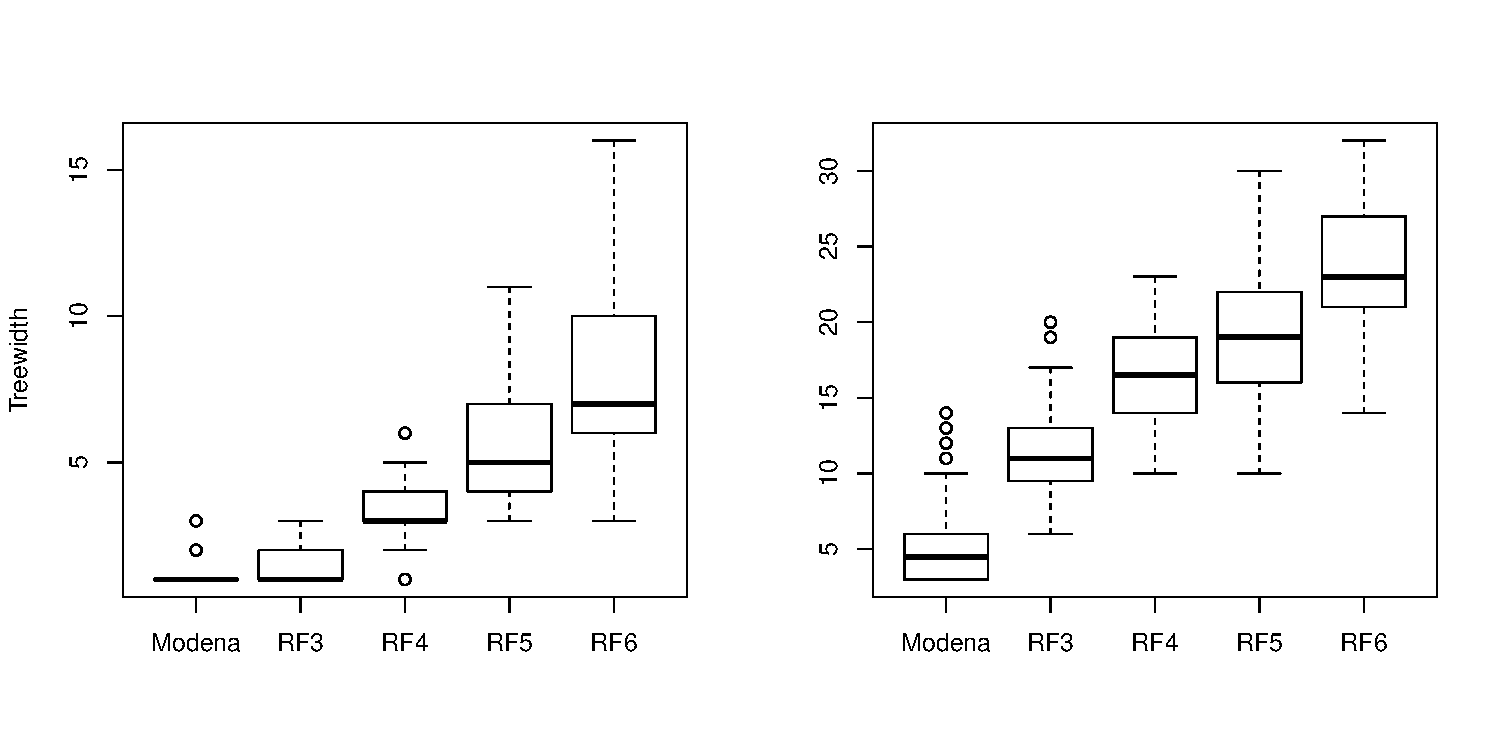
\includegraphics[width=0.9\textwidth]{Figs/td-widths}
  \caption{Treewidths for multi-target RNA design instances of
    different complexity. Distributions of treewidths shown as boxplots for the base pair (left) and stacking model (right).}
  \label{fig:td-widths}
\end{figure}

\begin{figure}
  %\hspace*{2cm}\textbf{Base pair model}\hspace{4.75cm}\textbf{Stacking model}\\[-28pt]
  \centering
  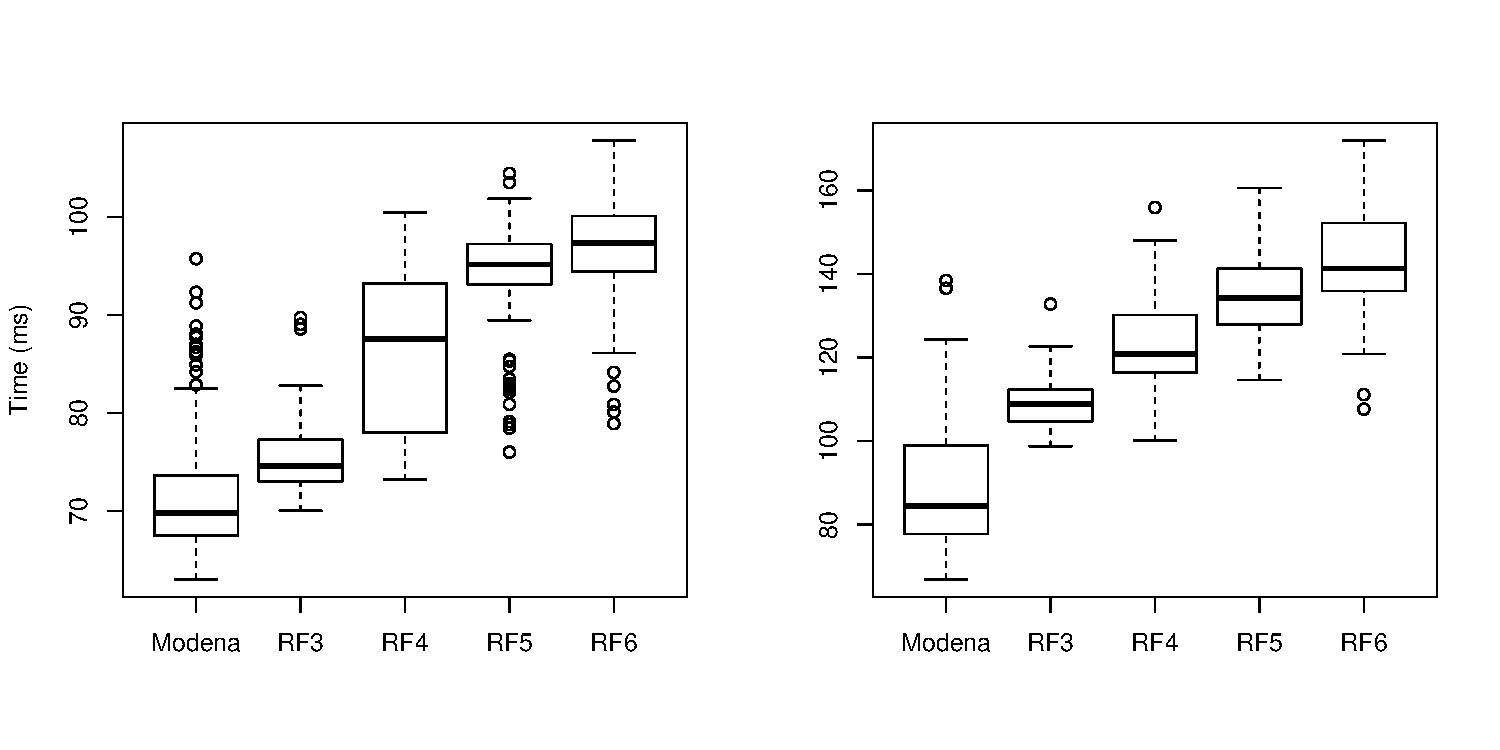
\includegraphics[width=0.9\textwidth]{Figs/td-times}
  \caption{Computation time of tree decompositions for
    multi-target RNA design instances of different complexity.
    Distributions of times (in ms/instance) shown as boxplots for the base pair (left) and stacking model (right).}
  \label{fig:td-times}
\end{figure}


\begin{figure}[t!]
  %% the figure shows benchmark_inputs/RNAfold/3str/f3.100.0.inp
  \centering
  \verbatiminput{Figs/f3_100_0.txt}
  \includegraphicstop[width=0.6\textwidth]{Figs/td-example-basepair}%
  \includegraphicstop[width=0.35\textwidth]{Figs/td-example-stacking}
  \caption{Example instance from RF3 (top) with its tree decompositions in the base pair (left) and stacking model (right). The respective treewidths are 2 and 12.}
  \label{fig:td-example}
\end{figure}

\section{Expressing higher arity functions as cliques in the dependency graph}
\label{appsec:dependency-cliques}

Our implementation relies on external tools for the tree decomposition. Therefore it is not trivial that the weight functions (i.e. terms of the energy function) can be captured within the tree decompositions returned by a specific tool. In other words, it is not immediately clear how one can construct a cluster tree from an arbitrary tree decomposition for a given network.

Crucially, one can show that, as long as the network the arguments $\dep(f)$ of a function $f$ are materialized by a clique within the network $\network$, then there exists at least one node in the tree decomposition that contains $\dep(f)$, thus allowing the evaluation of $f$.
\begin{lemma}\label{lem:cliques}
Let $G=(V,E)$ be an undirected graph, and  $T,\chi$ be a tree decomposition for $G$. For each clique $C\subset V$, there exists a node $n\in T$ such that $C\subset\chi(v)$.
\end{lemma}
\begin{proof}
  \newcommand{\TransVars}[1]{{\rm tverts}(#1)}
  \newcommand{\Children}[1]{{\rm Children}(#1)}
  For the sake of simplicity, let us consider $T$ as rooted on an arbitrary node, inducing an orientation, and denote by $\TransVars{n}\in V$ the set of vertices found in a node $n$ or its descendants, namely
    $$\TransVars{n} = \chi(n) \bigcup_{n'\in\Children{n}} \TransVars{n'}.$$

  Now consider (one of) the deepest node(s) $n\in T$, such that $C\subset\TransVars{v}$. We are going to prove that $C\subset\chi(n)$, using contradiction, by showing that $C\not\subset\chi(n)$ implies that $T$ is not a tree decomposition.

  Indeed, let us assume that $C\not\subset\chi(n)$, then there exists a node $v'\notin\chi(n)$ whose presence in $\TransVars{n}$ stems from its presence in some descendant of $n$. Let us denote by $n'\neq n$ the closest descendant of $n$ such that $v'\in\chi(n')$. Now, consider a node $v\in C$ such that $v\in \TransVars{v'}$ and $v\notin \TransVars{v'}$. Such a node always exists, otherwise $n'$, and not $n$, would be the deepest node such that $C\subset \TransVars{v'}$. From the definition of the tree decomposition, we know that neither $n'$ nor its descendants may contain $v$. On the other hand, none of the parents or siblings of $n'$ may contain $v'$. It follows that is no node $n''\in T$ whose vertex set $\chi(v'')$ includes, at the same time, $v$ and $v'$. Since both $v$ and $v'$ belong to a clique, one has $\{v,v'\}\in E$. The absence of a node in $T$ capturing an edge in $E$ contradicts our initial assumption that $T$ is tree decomposition for $G$.

  We conclude that $n$ is such that $C\not\subset\chi(n)$.
\end{proof}

This result implies that classic tree decomposition algorithms and, more importantly, implementations can be directly re-used to produce decompositions that capture energy models of arbitrary complexity, functions of arbitrary arity. Indeed, it suffices to add a clique, involving the parameters of the function, and Lemma~\ref{lem:cliques} guarantees that the tree decomposition will feature one node to which the function can be associated.


\section{Correctness of the FPT partition function algorithm}
\label{appsec:correctness}

\begin{theorem}[Correctness of Alg.~\ref{alg:pf}]
  \label{the:pfalgo-correctness}
  As computed by Alg.~\ref{alg:pf} for cluster tree $(T,\chi,\phi)$,
  the messages $\Message{u}{v}$, for all edges $u\to{}v\in T$, yield
  the partition functions of subtree of $u$ for the partial sequences
  $\val\in\partseqs(\separator{u}{v})$, i.e. the messages satisfy
  \begin{equation}
   \evalfor{\Message{u}{v}}{\val} = \sum_{\val'\in\partseqs(\chi(T_r(u))-\separator{u}{v})} \quad
   \prod_{f\in\phi(T_r(u))} \exp(-\beta \evalfor{f}{\substitute{\val'}{\val}}),\label{eq:pfalgo-correct}
 \end{equation}
 where $\chi(T_r(u))$ denotes all $\chi$-assigned positions of nodes in $T_r(u)$;
 respectively $\phi(T_r(u))$; all $\phi$-assigned functions.
%
\end{theorem}

\begin{proof}
  Note that in more concise notation, Alg.~\ref{alg:pf} computes
  messages such that
\begin{equation}
  \evalfor{\Message{u}{v}}{\val} := \sum_{\val'\in\partseqs(\difference{u}{v})}\quad
  \prod_{f\in \phi(u) } \exp(-\beta \evalfor{f}{\substitute{\val'}{\val}}) \prod_{(w\to{}u) \in T} \evalfor{\Message{w}{u}}{\substitute{\val'}{\val}}.\label{eq:messages}
\end{equation}

Proof by induction on $T$. If $u$ is a leaf, $\chi(r) = \chi(T_r(u))$,
there are no messages sent to $u$, and $\phi(u) = \phi(T_r(u));$ implying
Eq.~$(\ref{eq:pfalgo-correct}).$
%
Otherwise, since the algorithm traverses edges in postorder, $u$ received from its children
$w_1,\dots,w_q$ the messages $\Message{w_1}{u}, \dots, \Message{w_q}{u}$, which satisfy Eq.~$(\ref{eq:pfalgo-correct})$ (induction hypothesis). Let $\val\in\partseqs(\separator{u}{v})$; then, $\evalfor{\Message{u}{v}}{\val}$ is computed by the algorithm according to Eq.~$(\ref{eq:messages})$. We rewrite as follows
\begin{align*}
  & \sum_{\val'\in\partseqs(\difference{u}{v})}\quad
    \prod_{f\in \phi(u) } \exp(-\beta \evalfor{f}{\substitute{\val'}{\val}})
    \prod_{(w\to{}u) \in T} \evalfor{\Message{w}{u}}{\substitute{\val'}{\val}}\\
  & = \sum_{\val'\in\partseqs(\chi(u)-\separator{u}{v})}\quad
    \prod_{f\in \phi(u) } \exp(-\beta \evalfor{f}{\substitute{\val'}{\val}})
    \prod_{i=1}^q \evalfor{\Message{w_i}{u}}{\substitute{\val'}{\val}}\\
  & =_{IH}
    \sum_{\val'\in\partseqs(\chi(u)-\separator{u}{v})}\quad
    \prod_{f\in \phi(u) } \exp(-\beta \evalfor{f}{\substitute{\val'}{\val}})
    \prod_{i=1}^q \sum_{\val''\in\partseqs(\chi(T_r(w_i))-\separator{w_i}{u})} \quad
    \prod_{f\in\phi(T_r(w_i))} \exp(-\beta \evalfor{f}{\substitute{\val''}{\substitute{\val'}{\val}}}) \\
& =_{*}
    \sum_{\val'\in\partseqs(\chi(u)-\separator{u}{v})}\quad
  \sum_{\val''\in\partseqs(\bigcup_{i=1}^q\chi(T_r(w_i))-\separator{w_i}{u})} \quad
  \prod_{f\in \phi(u) } \exp(-\beta \evalfor{f}{\substitute{\val'}{\val}})
  \prod_{f\in\phi(T_r(w_i))} \exp(-\beta \evalfor{f}{\substitute{\val''}{\val'} | \val}) \\
  & =_{(**)} \sum_{\val'\in\partseqs(\chi(T_r(u))-\separator{u}{v})}\quad
    \prod_{f\in \phi(T_r(u)) } \exp(-\beta \evalfor{f}{\substitute{\val'}{\val}})\\
\end{align*}
To see (*) and (**), we observe:
\begin{itemize}
\item The sets $\chi(u)-\separator{u}{v}$ and
  $\chi(T_r(w_i))-\separator{w_i}{u}$ are all disjoint due to
  Def.~\ref{def:treedecomp}, property 2. First, this property implies
  that any shared position between the subtrees of $w_i$ and $w_j$
  must be in $\chi(w_i)$, $\chi(w_j)$ and $\chi(u)$, thus the
  positions of $\chi(T_r(w_i))-\separator{w_i}{u}$ are
  disjoint. Second, if a position $\chi(T_r(w_i))$ occurs in
  $\chi(u)$, it must occur in $\chi(w_i)$ and consequently in $\separator{u}{v}$.
\item The union of the sets $\chi(u)-\separator{u}{v}$ and
  $\chi(T_r(w_i))-\separator{w_i}{u}$ is $\chi(T_r(u))-\separator{u}{v}).$
\end{itemize}

\end{proof}

\section{General complexity of the partition function computation by cluster tree elimination and generation of samples}
\label{appsec:algcomplexity}

\begin{proposition}
  \label{prop:general-complexity}
Given a cluster tree $(T,\chi,\phi)$, $T=(V,E)$ of the RNA design network $\network=(\X,\F)$ with treewidth $w$ and maximum separator size $s$, computing the partition function by Algorithm~\ref{alg:pf} takes $O((|F|+|V|)\cdot 4^{w+1})$ time and $O(|V| 4^s)$ space (for storing all messages). The sampling step has time complexity of $O((|F|+|V|)\cdot 4^D)$ per sample.
\end{proposition}

\begin{proof}[Proposition~\ref{prop:general-complexity}]
Let $d_u$ denote the degree of node $u$ in $T$, $s_u$ is the size of the separator between
$u$ and its parent in $T$ rooted at $r$. For each node in the cluster tree, Alg.~\ref{alg:pf} computes one message by combining $(|\phi(u)|+d_u-1)$ functions, each time enumerating $4^{|\chi(u)|}$ combinations; Alg.~\ref{alg:sampling} computes $4^{|\chi{u}|-s_u}$ partition functions each time combining $(|\phi(u)|+d_u-1)$ functions.  $4^{|\chi(u)|}$ is bound by $4^{w+1}$ and $4^{|\chi{u}|-s_u}$ by $4^D$; moreover $\sum_{u\in V} (|\phi(u)|+d_u-1) = |F|+|V|-1$.
\end{proof}


\section{Exploiting constraint consistency to reduce the complexity}\label{sec:improvedComplexity}

%\textcolor{red}{\textbf{SW: Simpler alternative to
%    Sec.~\ref{sec:first-improvedComplexity}. Note also that the use of
%    variables in Sec.~\ref{sec:first-improvedComplexity} conflicts
%    with the (recent) specialization of constraint networks to RNA design
%    networks.}}

While Alg.~\ref{alg:pf} computes messages values for
\emph{all} possible combinations of nucleotides for the positions 
% in the separator set, 
% yp: for all the positions in a node, right?
in a node, 
we observe here that many such combinations are \emph{not} required for computing all relevant
partition functions. In particular, the algorithm can be restricted to
consider only \Def{valid} combinations, satisfying the (hard)
constraints induced by valid base pairs.

RNA design introduces constraints due to the requirement of canonical
(aka complementary) base pairing, which can be exploited in a
particularly simple and effective way to reduce the complexity.  
As previously noted by \citet{Flamm2001}, the base pair complementarity induces a
bi-partition of each connected component within the base pair
dependency graph, such that the nucleotides assigned to the two set of
nodes in the partition are restricted to values in $\{\Ab,\Gb\}$ and
$\{\Cb,\Ub\}$ respectively. We call a partial sequence
\Def{cc-valid}, iff its determined positions are consistent with such a separation
for all determined positions of the same connected component.

% Let $CC=\{cc_1$, $cc_2, \dots\}$ denote the vertex sets of the
% connected components of the base pair dependency graph. In this graph,
% let each component have the bi-partition $cc_i=cc^0_i\cup cc^1_i$.

One can now modify Alg.~\ref{alg:pf}, on a tree decomposition
$(T,\chi)$, such that the message values
$\evalfor{\Message{u}{v}}{\val}$ are only computed for cc-valid
partial sequences $\val\in\partseqs(\separator{u}{v})$. Moreover, the
loop over $\val'\in\partseqs(\difference{u}{v})$ is restricted, such
that $\substitute{\val}{\val'}$ are cc-valid. Analogous restrictions are 
then implemented in the sampling algorithm Alg.~\ref{alg:sampling}.

The correctness of the modified algorithm follows from the same
induction argument, where the message computation over one node
evaluates messages from its children only at cc-valid partial
sequences. The result of this computation is a message, which corresponds 
to the partition function, restricted to cc-valid partial sequences. 
Since invalid sequences have infinite energy, they do not contribute to 
the partition function, and the partition function restricted to cc-valid sequences coincides 
with the initial one.



This restriction drastically improves the time
complexity. Indeed, for any given node $v$, the original algorithm sends message for 
 $\chi(v):=\substitute{\val}{\val'}$ such that
$\val\in\partseqs(\separator{u}{v})$ and
$\val'\in\partseqs(\difference{u}{v})$, while the modified algorithm
only considers cc-valid assignments for $\chi(v)$. Remark that, in any connected component $cc$, 
assigning some nucleotide to a position reduces cc-valid assignments to (at most) 
two alternatives for each of the $|cc|-1$ remaining positions. It follows that, for a node $v$ featuring positions from $\#cc(v)$ distinct connected components $\{cc_1,cc_2\ldots\}$ in the base pair dependency graph, the number of cc-valid assignments to positions in $\chi(v)$ is exactly
$$4^{\#cc(v)}\prod_{i=1}^{\#cc(v)} 2^{|cc_i|-1} = 2^{\#cc(v)}\, 2^{|\chi(v)|} \in \Theta(2^{\#cc}\, 2^{w+1}),$$
for a single node, where $\#cc$ is the total number of connected components in the base pair dependency graph, and $w$ is the tree-width of the tree decomposition $T$. Since the number of nodes in $T$ is in $\Theta(n)$, and the number of atomic energy contributions associated with $k$ structures is in $\mathcal{O}(k\,n)$, then the overall complexity grows like $\Theta(n\, k\, 2^{\#cc}\, 2^{w+1})$.

%For each connected component having at least a position $i$ in $\chi(v)$, 
%the algorithm considers assigning any possible nucleotide $x\in \Sigma$ to $i$ and restricts
% the assignment of  for 
%any remaining position $j$ of the same connected component, it restricts the domain of $j$ to base-pairs that are consistent with the parity . 
%
%
%Let $c(v)$ be the number of connected components involving positions
%in $\chi(v)$; then, the first stage enumerates $2^{c(v)}$
%combinations. For each such combination, the second stage enumerates
%only $2^{|\chi(v)|}$ partial sequences, since there remain only two
%possible nucleotide choices for each position. All message values for
%node $v$ are thus computed in time
%$\Theta(2^{c(v)+|\chi(v)|})$. Consequently, the total time complexity
%of the modified algorithm is $$O(nk2^{\hat w}),$$ where $n$ is the RNA
%length, $k$ is the number of structures, and
%$\hat w := \max_{v\in T} c(v)+|\chi(v)|$.
%%
%From this directly follows the slightly looser complexity
%bound $$O(nk2^{w+1}2^{c})$$ in terms of treewidth $w$ and the maximum
%number $c$ of connected components represented in a node of the tree
%decomposition.  Notably, $\hat w$, as well as $w+1+c$, can not exceed
%$2(w+1)$, since $c\leq w+1$. Consequently the modified algorithm does
%never increase the original complexity.

Finally, we remark that even stronger time savings could be possible
in practice, since cc-valid partial sequences can still violate
complementarity constraints, e.g. by assigning C and A to positions in
different sets of a partition, thus satisfying the bi-partition
constraints, where the positions base pair directly, rendering the
partial sequence invalid. Moreover, applications of the sampling
framework, can introduce additional constraints that further reduce
the number of valid partial subsequences. However, exploiting all such
constraints, in a complete and general way, would likely cause significant
implementation overhead, while not significantly improving
the asymptotic complexity.


%\section{Exploiting the bipartite nature of base pair dependency
%  graphs to reduce the complexity}\label{sec:first-improvedComplexity}
%\textcolor{red}{\textbf{TODO: discuss and merge with/replace by previous Section}}
%
%As already noted by \citet{Flamm2001}, the requirement of canonical
%base pairing induces a bi-partition of each connected component within
%the base pair dependency graph, such that the nucleotides assigned to
%the two set of nodes in the partition are restricted to values
%$\{\Ab,\Gb\}$ and $\{\Cb,\Ub\}$ respectively.
%%
%It follows that, within each connected component of the base pair
%dependency graph, the assignment of any position drastically restricts
%the domain of the remaining positions, \emph{i.e.} they may now be
%assigned to only 2 out of the original 4 nucleotides.
%\newcommand{\Parity}[1]{p_{#1}} To exploit this property, and further
%reduce the exponential factor of the complexity, we introduce the
%notion of \Def{parity} of a vertex/position, whereby vertices of
%\Def{even} (resp. \Def{odd}) polarities may only be assigned values in
%$\{\Ab,\Gb\}$ (resp. $\{\Cb,\Ub\}$). Neighbors of an odd vertex must
%be even and vice versa, so the choice of a parity for any single
%vertex caracterizes the parity of all vertices in a bipartite
%connected subgraph.
%
%Let $CC=\{cc_1,cc_2,\ldots\}$ denote the connected components of the base pair dependency graph, we consider a modified version of the cluster tree, obtained by:
%\begin{enumerate}
%\item Electing, in each connected component $cc_i$, the first position $v_i^\star$ from the component encountered from the root in a pre-order traversal of the cluster tree;\label{step:election}
%\item Introducing new variables $\mathcal{P}=\{\Parity{1},\ldots,\Parity{|CC|}\}$, representing the parity of elected vertices;
%\item Adding, to each node $x$ in the tree decomposition, the parity variables of connected components that are represented in the node, \emph{i.e.} such that at least one of the positions in the connected component is in $\chi(x)$; \label{step:addparities}
%\item Introducing, in the tree decomposition, a chain of intermediate nodes to fix cases where more than a single (parity) variable is introduced between a parent and its child.\label{step:intermediates}
%\end{enumerate}
%Note that, since connected components correspond to connected subtrees in the tree decomposition, then adding those variables preserves the properties of a tree decomposition. Also, each node in the former cluster tree introduces at most one new variable compared to its parent, so the elected node is uniquely defined by the rule stated in Step~\ref{step:election}. Finally, we note that the parity of a variable $v\in cc_i$ is entirely characterized by the parity $\Parity{i}$ of $v_i^\star$, and the parity of the distance between $v$ and $v_i^\star$ in the base pair dependency graph. Namely, the parity of $v$ is $\Parity{i}$ if the distance between $v$ and $v^{\star}_i$ is even, and opposite to $\Parity{i}$ if odd. It follows that, thanks to the new variables introduced in Step~\ref{step:addparities}, the domain of each of the original variables can be reduced to two alternatives instead of the original four.
%
%The computation of Alg.~\ref{alg:pf} on the new cluster tree, considering reduced assignments for position variables and additional odd/even assignments for parity variables, has complexity in $\mathcal{O}(n\,k\,2^{w+1}\,2^{c})$, where $n$ is the RNA length, $k$ is the number of structures, $w$ is the tree-width of the unmodified cluster tree, and $c$ is the maximum number of connected components represented in a node. It should be noted that $c\le \min(|CC|,w+1)$, so that the new complexity cannot be larger than the one stated in Th.~\ref{th:complexities}. Also, note that the number of nodes introduced by Step~\ref{step:intermediates} is bounded by $|CC|$, so that the introduction of these intermediate nodes does not impact the worst-case complexity. For the same reason, the complexity of the stochastic backtrack remains unchanged.

\section{Parameters for the base pair and the stacking energy model}
\label{appsec:modelparameters}

We trained parameters for two RNA energy models to approximate the
Turner energy model, as implemented in the \Software{ViennaRNA}
package.  In the \Def{base pair model}, the total energy of a sequence $S$
for an RNA structure $R$ is given as sum of base pair energies, where
we consider six types of base pairs distinguishing by the bases $\Ab$-$\Ub$,
$\Cb$-$\Gb$ or $\Gb$-$\Ub$ (symmetrically) and between stacked and non-stacked base
pairs; here, we consider base pairs $(i,j)\in R$ \Def{stacked} iff
$(i+1,j-1)\in R$, otherwise \Def{non-stacked}. In the \Def{stacking model},
our features are defined by the stacks, i.e. pairs $(i,j)$ and
$(i+1,j-1)$ which both occur in $R$; we distinguish 18 types based on
$S_i,S_j,S_{i+1},S_{j-1}$ (i.e. all combinations that allow canonical
base pairs; the configurations $S_i,S_j,S_{i+1},S_{j-1}$ and
$S_{i+1},S_{j-1},S_j,S_i$ are symmetric).

Both models describe the energy assigned to a pair of sequence and
structure in linear dependency of the number of features and their
weights. We can thus train weights for linear predictors of the Turner
energy in both models.

For this purpose, we generated 5000 uniform random RNA sequences of
random lengths between 100 and 200. For each sample, we predict the
minimum free energy and corresponding structure using the ViennaRNA
package; then, we count the distinguished features (i.e., base pair or
stack types). The parameters are estimated fitting linear models
without intercept (\texttt{R} function \texttt{lm}). For both models,
\texttt{R} reports an adjusted R-squared value of 0.99. The resulting
parameters are reported in Tables~\ref{tab:basepairmodel} and
\ref{tab:stackingmodel}.

For validating the trained parameters, we generate a second
independent test set of random RNA sequences in the same
way. Fig.~\ref{fig:training-cor} shows correlation plots for the
trained parameters in the base pair and stacking models for predicting
the Turner energies in the test set with respective correlations of
$0.95$ an $0.94$.

\begin{figure}
  \centering
  A)\includegraphicstop[width=0.4\textwidth,trim=0 0 0 50,clip]{Figs/basepaircor}
  B)\includegraphicstop[width=0.4\textwidth,trim=0 0 0 50,clip]{Figs/stackingcor}
  \caption{Validation of the trained parameters for the A) base pair
    model B) stacking model for predicting energies of the
    independently sampled sequences in the test set. We show
    correlation plots against the Turner energies reported by the
    ViennaRNA package.}
  \label{fig:training-cor}
\end{figure}

\begin{table}[b]
  \centering
  \caption{Trained weights for the base pair energy model.}
  \label{tab:basepairmodel}
  \begin{tabular}{c@{\quad}c@{\quad}c@{\quad}|@{\quad}c@{\quad}c@{\quad}c}
    \multicolumn{3}{c}{non-stacked} & \multicolumn{3}{c}{stacked}\\
    AU      & CG       & GU      & AU       & GC       & GU \\\hline
    1.26630 & -0.09070 & 0.78566 & -0.52309 & -2.10208 & -0.88474
  \end{tabular}
\end{table}

% GC_IN = -0.09070;
% AU_IN = 1.26630;
% GU_IN = 0.78566;
% GC_TERM = -2.10208;
% AU_TERM = -0.52309;
% GU_TERM = -0.88474;

\begin{table}[b]
  \centering
  \caption{Trained weights for the stacking energy model (the rows specify $S_i,S_j$; the columns, $S_{i+1},S_{j-1}$; we do not show the symmetric weights).}
  \label{tab:stackingmodel}
  \begin{tabular}{c@{\quad}|@{\quad}c@{\quad}c@{\quad}c@{\quad}c@{\quad}c@{\quad}c@{\quad}c@{\quad}c}
       & AU & CG & GC & GU & UA & UG \\\hline
    AU &
-0.18826 &
-1.13291 &
-1.09787 &
-0.38606 &
-0.26510 &
-0.62086
    \\
    CG &
-1.11752 &
-2.23740 &
-1.89434 &
-1.22942 &
-1.10548 &
-1.44085
    \\
    GU &
-0.55066 &
-1.26209 &
-1.58478 &
-0.72185 &
-0.49625 &
-0.68876
    \\
  \end{tabular}
\end{table}

\section{Monotonicity of the partial derivatives within weight calibration}
\label{sec:weight_derivatives}
%
In weighted distributions, one witnesses a fairly predictable impact of the variation of any weight $\pi_\ell$ over the expected value $\mathbb{E}(E_\ell\mid \pmb{\pi})$, $\pmb{\pi}:= (\pi_1\cdots\pi_k)$, of the free energy $E_\ell$ of structure $\ell$.  Let us  first remind the probability of a sequence $S$ in the weighted distribution
\begin{align*}
  \mathcal{B}_{\pmb{\pi}}(S) &= \prod_{i=1}^{k} \pi_i^{-E_i(S)}, &
  \partfun{\pmb{\pi}}&=\sum_{S'}\mathcal{B}_{\pmb{\pi}}(S') &
    \text{and}& &
  \mathbb{P}(S\mid \pmb{\pi}) &= \frac{\mathcal{B}_{\pmb{\pi}}(S)}{\partfun{\pmb{\pi}}}.
  \end{align*}

Remind also the definition of the expectation of $E_\ell(S)$, for $S$ a Boltzmann-distributed sequence:
$$\mathbb{E}(E_\ell\mid \pmb{\pi}) = \sum_S E_\ell(S)\cdot \mathbb{P}(S\mid \pmb{\pi}).$$

We first remark that the partial derivative of $\mathcal{B}$ yields
\begin{align*}
  \frac{\partial \mathcal{B}_{\pmb{\pi}}(S)}{\partial \pi_\ell} = -E_\ell(S)\cdot \pi_\ell^{-E_\ell(S)-1}\prod_{\substack{i=1\\i\neq \ell}}^{k} \pi_i^{-E_i(S)} = \frac{-E_\ell(S)}{\pi_\ell}\cdot\mathcal{B}_{\pmb{\pi}}(S) = -E_\ell(S)\cdot \mathbb{P}(S\mid \pmb{\pi})\cdot \frac{\partfun{\pmb{\pi}}}{\pi_\ell }
\end{align*}
while the partial derivative of $\mathcal{Z}$ gives
\begin{align*}
  \frac{\partial \partfun{\pmb{\pi}}(S)}{\partial \pi_\ell} = \sum_{S'} -E_\ell(S')\cdot \mathbb{P}(S'\mid \pmb{\pi})\cdot \frac{\partfun{\pmb{\pi}}}{\pi_\ell }= -\mathbb{E}(E_\ell\mid \pmb{\pi})\cdot \frac{\partfun{\pmb{\pi}}}{\pi_\ell}.
\end{align*}
From these expressions, we conclude that
\begin{align*}
  \frac{\partial \mathbb{E}(E_\ell\mid \pmb{\pi})}{\partial \pi_\ell} &= \sum_S E_\ell(S)\cdot\frac{\partial \mathbb{P}(S\mid \pmb{\pi})}{\partial \pi_\ell}\\
  %
  & = \sum_S E_\ell(S)\left(\frac{\frac{\partial \mathcal{B}_{\pmb{\pi}}(S)}{\partial \pi_\ell}}{\mathcal{Z}_{\pmb{\pi}}} - \frac{\frac{\partial \mathcal{Z}_{\pmb{\pi}}}{\partial \pi_\ell}\cdot\mathcal{B}_{\pmb{\pi}}(S)}{\mathcal{Z}_{\pmb{\pi}}^2}\right)\\
  %
  & = \sum_S E_\ell(S)\left(\frac{-E_\ell(S)\cdot \mathbb{P}(S\mid \pmb{\pi})\cdot \frac{\mathcal{Z}_{\pmb{\pi}}}{\pi_\ell }}{\mathcal{Z}_{\pmb{\pi}}} + \frac{\mathbb{E}(E_\ell\mid \pmb{\pi})\cdot \frac{\mathcal{Z}_{\pmb{\pi}}}{\pi_\ell}\cdot\mathcal{B}_{\pmb{\pi}}(S)}{\mathcal{Z}_{\pmb{\pi}}^2}\right)\\
  %
  & = \sum_S - \frac{E_\ell(S)^2\cdot\mathbb{P}(S\mid \pmb{\pi})}{\pi_\ell} + \frac{\mathbb{E}(E_\ell\mid \pmb{\pi})}{\pi_\ell}\sum_S E_\ell(S)\cdot \mathbb{P}(S\mid \pmb{\pi})\\
  & = -\frac{\mathbb{E}(E_\ell^2\mid \pmb{\pi}) - \mathbb{E}(E_\ell\mid \pmb{\pi})^2}{\pi_\ell}
\end{align*}
In the numerator of the above expression, one recognizes the variance of the distribution of $E_\ell$.
Remark that a variance is always non-negative and, in our case, also strictly positive for $\pmb{\pi}$, $\pi_\ell>0$, as soon as there exist at least two distinct sequences $S$ and $S'$ such that $E_\ell(S)\neq E_\ell(S')$.
Moreover, weights are always positive so the partial derivative in $\pi_\ell$ is always positive. Ultimately, it is always possible to increase (resp. decrease) the expected free energy of a structure by simply decreasing (resp. increasing) its weight, supporting our weight optimization procedure.
\newpage
\section{Detailed result of quality analysis}\label{sec:validity}
N/A values correspond to data that could not be obtained by the time of this submission for two main reasons: In the case of the initial sampling (left columns), they correspond to instances which, in conjunction with an expressive energy model, resulted in very high tree-width, leading to unreasonable memory requirements incompatible with our available computing resources; The case of missing values after optimization  (right columns), they indicate situations where the initial optimization took too long ($\approx$ 1 day) and was killed.
\subsection{RNAtabupath (2 structures)}
{\relsize{-1}
\begin{longtable}{@{}cr@{\hspace{1em}}r@{\hspace{1em}}r@{\hspace{1em}}r@{\hspace{1em}}r@{\hspace{2em}}r@{\hspace{1em}}r@{\hspace{1em}}r@{\hspace{1em}}r@{\hspace{1em}}r@{}}
&\multicolumn{2}{c}{Boltzmann}&\multicolumn{2}{l}{Uniform}&&\multicolumn{2}{l}{\begin{minipage}[b]{1.8cm} Boltzmann\\Optimized\end{minipage}}&\multicolumn{2}{l}{\begin{minipage}[b]{1.8cm} Uniform\\Optimized\end{minipage}}&\\ \toprule
Name&Mean&StDev&Mean&StDev&\%Gain&Mean&StDev&Mean&StDev&\%Gain\\ \midrule
alpha\_operon&17.18&4.18&25.86&5.97&51&2.12&0.81&2.36&0.88&11\\
amv&14.37&2.90&27.26&5.65&90&3.67&0.90&4.27&1.08&16\\
attenuator&10.74&3.04&21.44&4.77&100&1.39&0.55&1.81&0.80&30\\
dsrA&11.77&2.58&18.23&4.62&55&3.71&0.94&3.80&0.95& 2\\
hdv&22.08&4.88&35.48&6.68&61&3.63&1.16&4.57&1.48&26\\
hiv&41.22&6.74&73.00&9.40&77&16.87&3.45&29.89&5.36&77\\
ms2&13.35&3.73&19.79&4.55&48&2.41&0.76&2.66&0.97&10\\
rb1&17.70&4.35&37.38&7.14&111&2.64&0.90&3.82&1.31&45\\
rb2&16.63&4.16&25.17&5.85&51&2.75&0.86&3.07&0.97&12\\
rb3&22.47&4.71&41.18&7.09&83&3.79&1.01&5.05&1.52&33\\
rb4&26.15&4.30&47.89&6.80&83&10.57&&11.80&1.82&12\\
rb5&30.52&5.45&54.24&7.76&78&6.10&1.97&9.22&2.78&51\\
ribD&49.84&7.01&81.27&9.07&63&20.47&3.17&31.01&4.47&51\\
s15&11.00&2.97&18.37&4.53&67&1.96&0.64&2.12&0.77& 8\\
sbox&25.05&4.84&50.03&8.04&100&6.34&1.49&8.90&2.19&40\\
spliced&9.65&2.98&17.60&4.39&82&2.13&0.44&2.41&0.59&13\\
sv11&20.98&4.66&36.83&6.91&76&N/A&N/A&4.20&1.12&N/A\\
thim&29.35&5.39&48.32&6.95&65&8.69&1.90&12.12&2.54&39\\
\midrule
Average&21.67&4.38&37.74&6.45&74&5.84&1.31&7.95&1.76&28\\\bottomrule
\end{longtable}}
\subsection{RNAdesign (3 structures)}
{\relsize{-1}
\begin{longtable}{@{}cr@{\hspace{1em}}r@{\hspace{1em}}r@{\hspace{1em}}r@{\hspace{1em}}r@{\hspace{2em}}r@{\hspace{1em}}r@{\hspace{1em}}r@{\hspace{1em}}r@{\hspace{1em}}r@{}}
&\multicolumn{2}{c}{Boltzmann}&\multicolumn{2}{l}{Uniform}&&\multicolumn{2}{l}{\begin{minipage}[b]{1.8cm} Boltzmann\\Optimized\end{minipage}}&\multicolumn{2}{l}{\begin{minipage}[b]{1.8cm} Uniform\\Optimized\end{minipage}}&\\ \toprule
Name&Mean&StDev&Mean&StDev&\%Gain&Mean&StDev&Mean&StDev&\%Gain\\\midrule
sq100&20.67&4.90&31.78&5.46&54&5.81&1.53&8.33&1.92&43\\
sq10&19.91&5.24&26.62&5.59&34&3.50&0.81&3.88&0.94&11\\
sq11&19.38&4.81&27.76&5.69&43&2.81&0.77&3.31&0.89&18\\
sq12&17.19&3.62&22.62&4.98&32&2.70&0.65&2.79&0.68& 3\\
sq13&18.54&3.95&29.95&5.56&62&10.24&2.18&16.63&3.13&62\\
sq14&21.49&4.23&37.82&5.55&76&7.25&1.63&9.90&2.10&37\\
sq15&21.91&3.78&36.32&5.13&66&11.15&1.75&15.49&2.34&39\\
sq16&15.99&4.22&27.70&5.58&73&2.51&0.69&2.96&0.94&18\\
sq17&20.71&3.72&33.62&5.33&62&5.83&1.08&7.36&1.49&26\\
sq18&19.64&3.91&35.26&5.13&80&5.83&1.41&7.97&2.00&37\\
sq19&14.78&3.33&28.64&5.34&94&3.84&0.77&4.66&1.04&21\\
sq1&14.85&3.84&21.89&5.48&47&2.02&0.65&2.20&0.69& 9\\
sq20&17.39&3.82&27.90&4.93&60&3.93&1.04&5.18&1.48&32\\
sq21&21.64&3.94&36.27&5.16&68&8.28&1.82&11.41&2.40&38\\
sq22&17.65&4.13&31.57&5.45&79&5.66&1.51&10.02&2.50&77\\
sq23&19.44&3.66&32.38&5.40&67&12.05&1.85&18.69&3.18&55\\
sq24&18.01&4.01&27.92&5.30&55&3.59&0.93&4.25&1.10&19\\
sq25&17.54&5.20&26.65&6.11&52&1.35&0.34&1.45&0.40& 7\\
sq26&17.63&4.47&24.46&5.64&39&3.11&0.62&3.38&0.68& 9\\
sq27&17.93&3.61&28.51&5.30&59&7.55&1.49&10.96&2.38&45\\
sq28&14.78&3.71&29.35&5.99&99&2.32&0.49&2.66&0.62&15\\
sq29&17.61&3.72&26.95&5.08&53&4.44&0.98&5.22&1.21&18\\
sq2&22.43&4.19&37.25&5.15&66&10.34&1.71&14.32&2.35&39\\
sq30&19.11&4.04&31.75&5.54&66&6.06&1.61&8.99&2.19&48\\
sq31&19.97&3.87&31.92&5.20&60&5.12&1.19&6.34&1.55&24\\
sq32&21.96&4.00&31.65&5.23&44&5.24&1.29&6.84&1.76&31\\
sq33&15.11&4.30&22.75&5.52&51&1.78&0.43&2.08&0.63&17\\
sq34&25.00&4.17&37.46&5.03&50&12.46&1.84&18.73&2.57&50\\
sq35&19.25&4.12&32.72&5.35&70&5.90&1.25&7.96&1.82&35\\
sq36&12.77&2.91&26.76&5.39&110&3.19&0.77&3.61&0.94&13\\
sq37&18.71&3.88&32.44&5.62&73&3.24&0.90&4.21&1.25&30\\
sq38&14.55&3.56&29.02&5.29&99&2.79&0.86&3.70&1.22&33\\
sq39&22.75&3.95&33.06&4.98&45&9.20&1.76&11.87&2.33&29\\
sq3&20.38&4.07&36.86&5.60&81&4.69&1.19&6.30&1.72&34\\
sq40&19.46&4.35&31.76&5.41&63&4.05&0.94&4.96&1.19&23\\
sq41&14.41&3.46&27.85&5.57&93&3.33&0.71&3.91&0.88&17\\
sq42&18.67&3.87&35.20&5.55&89&5.32&1.24&6.96&1.56&31\\
sq43&17.32&3.97&31.63&5.38&83&3.53&0.89&4.27&1.15&21\\
sq44&19.37&3.84&31.75&5.09&64&5.52&1.29&7.26&1.60&31\\
sq45&18.53&4.77&27.40&5.53&48&2.54&0.67&2.84&0.74&12\\
sq46&17.92&3.80&28.83&5.09&61&4.45&0.90&5.41&1.20&22\\
sq47&15.09&3.78&28.23&5.82&87&3.02&0.78&3.45&0.85&14\\
sq48&18.90&4.23&36.27&5.78&92&4.69&1.08&6.71&1.67&43\\
sq49&20.13&4.69&27.24&5.39&35&3.15&0.76&3.66&0.95&16\\
sq4&19.31&4.69&29.25&5.34&51&2.36&0.79&3.24&1.15&37\\
sq50&17.01&3.92&28.43&5.35&67&3.15&0.73&3.54&0.86&12\\
sq51&22.18&4.14&36.07&5.20&63&11.56&1.79&16.57&2.88&43\\
sq52&19.36&3.93&31.04&5.20&60&11.04&2.21&16.25&3.04&47\\
sq53&13.78&3.72&24.48&5.46&78&1.65&0.39&1.88&0.53&14\\
sq54&18.07&3.59&33.99&5.57&88&8.15&1.57&12.35&2.59&51\\
sq55&21.93&4.68&30.11&5.21&37&4.59&0.82&5.43&1.13&18\\
sq56&17.83&3.90&31.69&5.46&78&4.22&0.75&4.84&0.93&15\\
sq57&16.30&3.97&28.48&5.45&75&1.96&0.58&2.28&0.71&16\\
sq58&12.74&2.86&32.97&5.80&159&3.77&0.82&4.89&1.22&29\\
sq59&20.44&4.54&33.02&5.57&62&6.05&1.50&8.34&2.08&38\\
sq5&9.97&2.72&17.94&4.93&80&1.29&0.33&1.41&0.39& 9\\
sq60&22.64&4.85&36.86&5.46&63&6.90&1.62&11.07&2.33&60\\
sq61&14.45&3.78&30.82&6.03&113&3.07&0.76&3.83&1.01&25\\
sq62&21.08&5.02&35.27&5.35&67&9.76&1.67&16.93&2.79&73\\
sq63&13.44&3.60&27.20&5.63&102&1.58&0.36&1.85&0.53&17\\
sq64&19.21&3.87&34.88&5.24&82&6.10&1.53&9.45&2.29&55\\
sq65&19.33&4.53&27.51&5.15&42&13.95&2.94&19.40&3.61&39\\
sq66&18.18&3.70&30.79&5.12&69&6.93&1.42&10.05&2.03&45\\
sq67&20.63&3.41&37.06&5.18&80&16.11&1.97&27.21&3.40&69\\
sq68&23.09&4.33&33.33&5.08&44&N/A&N/A&9.23&1.94&N/A\\
sq69&18.79&3.58&35.06&5.21&87&10.77&1.94&18.38&3.00&71\\
sq6&20.32&3.77&38.48&5.48&89&5.55&1.32&8.63&2.04&56\\
sq70&13.59&3.31&31.06&5.52&129&2.59&0.80&3.80&1.17&47\\
sq71&20.07&4.05&32.71&5.39&63&5.57&1.06&6.61&1.30&19\\
sq72&15.02&3.22&24.48&4.94&63&2.02&0.57&2.49&0.84&23\\
sq73&14.88&3.74&28.44&5.56&91&2.34&0.69&3.10&1.04&32\\
sq74&17.80&4.10&30.13&5.30&69&4.12&0.79&5.03&1.04&22\\
sq75&19.66&4.05&31.19&5.19&59&5.63&1.26&7.52&1.70&34\\
sq76&19.91&3.84&32.44&5.12&63&9.12&1.92&13.89&2.39&52\\
sq77&18.69&3.46&34.83&5.21&86&6.01&1.25&8.61&1.75&43\\
sq78&18.28&3.48&32.94&6.01&80&5.39&1.12&7.07&1.51&31\\
sq79&21.57&4.71&30.73&5.47&42&13.10&2.89&17.86&3.45&36\\
sq7&20.28&3.76&32.95&5.41&63&5.51&1.70&6.68&1.90&21\\
sq80&15.62&3.92&28.29&5.30&81&1.85&0.53&2.41&0.88&30\\
sq81&21.24&4.57&29.92&5.44&41&3.74&0.95&4.67&1.33&25\\
sq82&8.85&2.35&19.89&5.36&125&1.39&0.21&1.47&0.28& 6\\
sq83&14.13&3.60&28.92&5.45&105&2.77&0.76&3.52&1.01&27\\
sq84&15.60&3.98&24.12&5.26&55&2.54&0.47&2.85&0.65&12\\
sq85&15.56&3.39&26.09&5.18&68&2.19&0.62&2.70&0.82&23\\
sq86&21.54&4.95&34.21&5.77&59&4.66&1.21&5.92&1.51&27\\
sq87&16.45&3.85&32.65&5.81&98&3.50&0.62&4.14&0.86&18\\
sq88&20.05&5.09&33.45&5.86&67&2.50&0.72&3.17&0.99&27\\
sq89&14.77&4.20&26.15&5.59&77&1.79&0.50&2.01&0.62&13\\
sq8&15.85&4.14&30.34&6.02&91&2.85&0.79&3.85&1.15&35\\
sq90&15.25&3.99&29.83&5.80&96&2.10&0.64&2.90&1.06&38\\
sq91&17.29&3.93&27.19&5.08&57&3.69&1.11&4.48&1.31&21\\
sq92&19.06&3.57&33.07&5.34&74&4.77&1.11&6.83&1.78&43\\
sq93&19.48&4.11&29.17&5.65&50&3.29&0.80&3.86&1.03&17\\
sq94&14.72&3.21&27.05&5.43&84&3.98&0.77&4.66&0.98&17\\
sq95&17.60&3.72&33.42&5.38&90&12.86&2.20&22.76&3.84&77\\
sq96&15.35&3.84&31.62&5.68&106&2.69&0.67&3.52&1.02&31\\
sq97&18.28&3.89&29.22&5.03&60&4.31&1.13&5.32&1.42&23\\
sq98&18.84&4.57&29.30&5.42&56&2.78&0.73&3.59&0.97&29\\
sq99&19.74&4.19&30.95&5.28&57&3.94&0.98&4.89&1.33&24\\
sq9&17.30&4.26&26.15&5.72&51&1.66&0.44&1.79&0.55&8\\
\midrule
Average&21.67&4.38&37.74&6.45&74&5.84&1.31&7.95&1.76&28\\\bottomrule
\end{longtable}}
\subsection{RNAdesign (4 structures)}
{\relsize{-1}
\begin{longtable}{@{}cr@{\hspace{1em}}r@{\hspace{1em}}r@{\hspace{1em}}r@{\hspace{1em}}r@{\hspace{2em}}r@{\hspace{1em}}r@{\hspace{1em}}r@{\hspace{1em}}r@{\hspace{1em}}r@{}}
&\multicolumn{2}{c}{Boltzmann}&\multicolumn{2}{l}{Uniform}&&\multicolumn{2}{l}{\begin{minipage}[b]{1.8cm} Boltzmann\\Optimized\end{minipage}}&\multicolumn{2}{l}{\begin{minipage}[b]{1.8cm} Uniform\\Optimized\end{minipage}}&\\ \toprule
Name&Mean&StDev&Mean&StDev&\%Gain&Mean&StDev&Mean&StDev&\%Gain\\\midrule
sq100&21.70&4.41&33.19&4.93&53&12.52&2.62&17.14&3.10&37\\
sq10&20.66&5.16&27.00&5.24&31&N/A&N/A&8.02&2.05&N/A\\
sq11&22.23&4.23&30.73&5.31&38&6.09&1.21&7.70&1.70&26\\
sq12&18.30&3.55&23.38&4.93&28&3.75&0.53&3.94&0.64& 5\\
sq13&21.01&3.57&31.66&4.93&51&15.63&1.69&21.61&2.69&38\\
sq14&22.44&3.16&39.77&5.28&77&17.56&2.21&25.04&3.21&43\\
sq15&22.66&3.72&36.31&5.01&60&17.45&2.38&26.80&3.34&54\\
sq16&18.22&4.12&28.54&5.33&57&3.27&0.74&3.78&0.90&16\\
sq17&23.04&4.01&35.87&5.28&56&12.76&2.54&18.43&2.86&44\\
sq18&21.20&3.49&35.78&5.39&69&8.15&1.47&10.75&2.02&32\\
sq19&15.36&2.73&32.12&4.95&109&13.22&1.73&23.64&3.41&79\\
sq1&15.14&3.83&22.32&5.28&47&2.55&0.56&2.66&0.56& 4\\
sq20&16.75&3.09&29.25&4.74&75&9.26&1.67&13.40&2.41&45\\
sq21&23.98&3.72&38.18&5.14&59&16.15&2.10&23.31&3.16&44\\
sq22&20.38&3.81&32.90&5.12&61&8.42&1.44&12.39&2.03&47\\
sq23&18.39&3.36&32.82&5.34&78&12.07&1.93&19.58&3.26&62\\
sq24&20.05&4.10&29.72&5.29&48&5.40&1.15&7.28&1.68&35\\
sq25&21.48&5.35&28.83&5.78&34&2.95&0.66&3.30&0.77&12\\
sq26&20.83&4.63&27.39&5.25&32&4.20&0.76&4.80&0.96&14\\
sq27&17.14&3.48&29.41&5.24&72&7.58&1.45&11.67&2.34&54\\
sq28&23.50&4.48&33.84&6.07&44&5.59&1.03&6.69&1.39&20\\
sq29&18.14&3.65&27.22&4.85&50&5.54&0.92&6.26&1.17&13\\
sq2&N/A&N/A&N/A&N/A&N/A&N/A&N/A&N/A&N/A&N/A\\
sq30&19.40&3.76&32.40&4.95&67&8.89&1.56&12.39&2.19&39\\
sq31&24.97&3.80&32.68&5.19&31&8.77&1.18&13.05&2.15&49\\
sq32&19.62&3.76&31.03&4.97&58&5.50&1.29&7.57&1.71&38\\
sq33&19.51&4.25&27.65&5.12&42&4.23&0.91&5.37&1.16&27\\
sq34&25.60&3.50&37.58&4.90&47&13.41&1.77&20.62&2.68&54\\
sq35&21.87&3.93&35.50&5.73&62&9.66&1.56&13.80&2.31&43\\
sq36&11.65&2.59&26.29&5.48&126&3.33&0.60&3.86&0.90&16\\
sq37&25.80&4.48&36.19&4.90&40&15.84&2.03&23.46&2.85&48\\
sq38&17.74&3.43&32.11&5.14&81&4.95&0.93&6.20&1.38&25\\
sq39&21.54&3.83&32.74&5.21&52&9.79&1.81&13.10&2.29&34\\
sq3&20.19&4.06&39.87&5.23&97&14.60&2.26&26.21&3.32&79\\
sq40&18.68&4.18&33.41&5.62&79&4.32&0.92&5.49&1.30&27\\
sq41&15.86&3.46&30.06&5.30&89&5.56&0.94&6.59&1.17&19\\
sq42&21.79&3.25&38.72&5.11&78&N/A&N/A&23.27&3.45&N/A\\
sq43&23.21&3.99&33.89&5.33&46&7.27&1.30&9.08&1.76&25\\
sq44&21.65&3.59&33.47&4.99&55&8.04&1.42&10.91&1.97&36\\
sq45&19.01&4.79&27.79&5.58&46&3.45&0.65&3.81&0.83&10\\
sq46&20.08&3.60&30.69&4.89&53&7.68&1.30&9.96&1.69&30\\
sq47&17.29&3.73&29.94&5.26&73&4.52&1.03&5.24&1.20&16\\
sq48&28.78&4.03&38.24&5.57&33&16.87&1.76&25.52&3.19&51\\
sq49&19.19&4.75&27.33&5.42&42&3.14&0.73&3.66&0.86&17\\
sq4&19.71&4.46&29.44&5.30&49&3.35&0.87&4.25&1.18&27\\
sq50&19.36&4.11&30.60&5.49&58&4.99&0.79&5.71&0.98&14\\
sq51&N/A&N/A&38.68&5.02&N/A&N/A&N/A&27.99&2.48&N/A\\
sq52&21.40&3.37&33.80&5.43&58&16.30&2.43&25.10&3.67&54\\
sq53&15.81&3.50&28.75&5.32&82&4.29&1.05&6.22&1.53&45\\
sq54&18.16&3.45&35.10&4.86&93&15.32&2.23&26.27&3.37&71\\
sq55&22.47&4.43&31.94&5.15&42&11.05&2.41&15.19&2.98&37\\
sq56&21.11&4.12&35.25&5.93&67&12.27&2.00&18.68&2.97&52\\
sq57&18.94&3.91&30.86&5.51&63&3.69&0.71&4.51&0.90&22\\
sq58&19.68&2.97&35.80&5.41&82&9.78&1.44&16.76&2.66&71\\
sq59&20.35&3.75&33.08&5.20&63&17.24&2.82&24.28&3.93&41\\
sq5&11.60&2.54&19.61&5.12&69&1.92&0.35&2.12&0.49&11\\
sq60&21.97&4.37&38.39&5.44&75&17.44&2.44&29.57&3.89&70\\
sq61&19.07&3.46&34.14&5.24&79&6.90&1.33&10.30&1.97&49\\
sq62&25.71&5.09&34.50&4.88&34&12.33&1.94&17.33&2.62&41\\
sq63&17.21&3.45&30.71&5.37&78&5.49&1.36&7.38&1.84&34\\
sq64&19.89&3.52&35.51&4.96&79&14.00&2.12&22.04&3.12&57\\
sq65&18.69&4.06&29.18&5.34&56&12.55&2.26&17.63&2.94&41\\
sq66&17.50&3.40&30.59&5.16&75&8.71&1.62&13.67&2.43&57\\
sq67&22.63&4.21&36.73&5.06&62&17.17&2.21&26.90&3.34&57\\
sq68&N/A&N/A&35.00&5.13&N/A&N/A&N/A&17.96&2.39&N/A\\
sq69&N/A&N/A&36.07&4.91&N/A&N/A&N/A&24.53&2.08&N/A\\
sq6&22.32&3.77&40.27&5.41&80&6.25&1.39&9.46&2.08&51\\
sq70&16.97&4.07&31.84&5.51&88&3.64&0.88&5.09&1.32&40\\
sq71&19.34&4.07&31.81&5.24&64&5.09&0.95&6.26&1.20&23\\
sq72&16.60&3.01&29.22&4.92&76&6.20&1.18&7.67&1.57&24\\
sq73&18.64&3.44&30.86&5.16&66&12.54&2.35&21.15&4.05&69\\
sq74&17.24&3.88&31.19&5.47&81&13.12&3.31&21.49&4.11&64\\
sq75&18.44&3.60&31.25&5.19&70&7.24&1.37&11.19&2.21&55\\
sq76&20.76&3.38&33.74&4.94&63&16.90&2.38&25.18&3.38&49\\
sq77&21.92&3.29&35.83&5.26&63&10.59&1.63&13.96&2.25&32\\
sq78&23.60&3.17&36.23&5.47&54&19.14&2.52&26.07&3.61&36\\
sq79&24.77&4.43&32.49&5.23&31&18.07&2.89&23.78&3.64&32\\
sq7&19.94&3.54&32.78&5.29&64&5.37&1.65&6.59&1.89&23\\
sq80&18.63&3.88&29.75&5.27&60&2.87&0.64&3.64&1.01&26\\
sq81&23.57&3.63&36.02&5.24&53&17.71&2.20&25.76&3.17&45\\
sq82&13.21&3.25&25.45&5.00&93&3.05&0.67&4.06&1.00&33\\
sq83&14.37&3.21&31.96&5.41&122&3.86&0.84&5.55&1.31&44\\
sq84&19.05&3.89&29.35&5.00&54&5.21&0.99&6.38&1.32&23\\
sq85&17.32&3.91&30.80&5.43&78&10.61&2.09&17.53&2.93&65\\
sq86&25.19&4.04&36.79&5.66&46&9.04&1.93&14.14&2.62&56\\
sq87&16.91&3.89&32.84&5.34&94&4.94&0.79&6.08&1.18&23\\
sq88&22.92&4.99&35.87&5.65&56&5.22&1.00&6.58&1.30&26\\
sq89&17.52&3.91&29.24&5.45&67&4.14&0.86&4.83&1.11&17\\
sq8&25.56&4.49&33.42&5.21&31&N/A&N/A&12.55&2.05&N/A\\
sq90&18.67&3.62&33.21&5.33&78&5.40&0.98&7.26&1.62&34\\
sq91&18.00&3.83&26.82&4.85&49&8.01&1.72&11.08&2.41&38\\
sq92&20.51&3.28&37.62&4.84&N/A&17.62&2.17&29.08&3.47&65\\
sq93&22.63&4.66&33.40&5.25&48&11.43&2.16&16.37&3.00&43\\
sq94&14.71&3.25&28.06&5.39&91&3.81&0.72&4.51&0.97&18\\
sq95&N/A&N/A&36.93&5.11&N/A&N/A&N/A&23.98&2.67&N/A\\
sq96&17.20&3.70&33.01&5.46&92&5.98&1.20&8.09&1.71&35\\
sq97&19.78&3.85&30.01&5.09&52&6.05&1.25&7.45&1.60&23\\
sq98&21.39&4.33&31.13&5.16&46&4.77&0.77&5.67&1.03&19\\
sq99&20.33&4.39&29.97&5.07&47&4.05&1.07&4.95&1.28&22\\
sq9&18.86&4.22&29.51&5.22&56&3.93&0.88&5.06&1.35&29\\
\\\midrule
Average&19.94&3.84&32.29&5.24&63&8.77&1.48&13.13&2.13&37\\ \bottomrule
\end{longtable}}


\bibliographystyle{natbib}
%\bibliographystyle{achemnat}
%\bibliographystyle{plainnat}
%\bibliographystyle{abbrv}
%\bibliographystyle{bioinformatics}
%
%\bibliographystyle{plain}
%
\bibliography{biblio}


\end{document}